\cleardoublepage



\chapter{Résultats - Discussion}

%%%%%%%%%%%%%%%%%%%%%%%%%%%%%%%%%%%%%%%%%%%%%%%%%%%%%%%%%%%%%%%%%%%%%%%%%%%%%%%%%%%%%%%%%%%%%%%%%%%%
%%%%%%%%%%%%%%%%%%%%%%%%%%%%%%%%%%%%%%%%%%%%%%%%%%%%%%%%%%%%%%%%%%%%%%%%%%%%%%%%%%%%%%%%%%%%%%%%%%%%
%%%%%%%%%%%%%%%%%%%%%%%%%%%%%%%%%%%%%%%%%%%%%%%%%%%%%%%%%%%%%%%%%%%%%%%%%%%%%%%%%%%%%%%%%%%%%%%%%%%%
%%%%%%%%%%%%%%%%%%%%%%%%%%%%%%%%%%%%%%%%%%%%%%%%%%%%%%%%%%%%%%%%%%%%%%%%%%%%%%%%%%%%%%%%%%%%%%%%%%%%
%%%%%%%%%%%%%%%%%%%%%%%%%%%%%%%%%%%%%%%%%%%%%%%%%%%%%%%%%%%%%%%%%%%%%%%%%%%%%%%%%%%%%%%%%%%%%%%%%%%%

\section{Manipulation des machines virtuelles}
\label{Manipulation des machines virtuelles}

Les différentes classes développées en Python permettent la paramétrisation et le contrôle des machines virtuelles de type VirtualBox.
Les fonctionnalités principalement utilisées dans la solution sont :
\begin{itemize}
	\item Paramétrisation de la machine virtuelle : nombre de CPU, quantité de RAM ;
	\item Intervention sur l'état de la machine virtuelle : démarrage, mise en pause, arrêt ;
	\item Gestion des disques virtuels : ajout, retrait, montage et démontage dans Linux ;
	\item Gestion des répertoires partagés : partage, montage et démontage dans Linux ;
	\item Gestion de l'arborescence de Linux : création de répertoire, suppression de fichiers ou répertoires, copie ;
	\item Gestion des processus fonctionnant dans la machine virtuelle : pause, reprise et arrêt ;
	\item Échanges de fichiers ou répertoires entre la machine hôte et la machine virtuelle.
\\
\end{itemize}





%%%%%%%%%%%%%%%%%%%%%%%%%%%%%%%%%%%%%%%%%%%%%%%%%%%%%%%%%%%%%%%%%%%%%%%%%%%%%%%%%%%%%%%%%%%%%%%%%%%%
%%%%%%%%%%%%%%%%%%%%%%%%%%%%%%%%%%%%%%%%%%%%%%%%%%%%%%%%%%%%%%%%%%%%%%%%%%%%%%%%%%%%%%%%%%%%%%%%%%%%
%%%%%%%%%%%%%%%%%%%%%%%%%%%%%%%%%%%%%%%%%%%%%%%%%%%%%%%%%%%%%%%%%%%%%%%%%%%%%%%%%%%%%%%%%%%%%%%%%%%%
%%%%%%%%%%%%%%%%%%%%%%%%%%%%%%%%%%%%%%%%%%%%%%%%%%%%%%%%%%%%%%%%%%%%%%%%%%%%%%%%%%%%%%%%%%%%%%%%%%%%
%%%%%%%%%%%%%%%%%%%%%%%%%%%%%%%%%%%%%%%%%%%%%%%%%%%%%%%%%%%%%%%%%%%%%%%%%%%%%%%%%%%%%%%%%%%%%%%%%%%%

\section{L'interface graphique utilisateur}

%%%%%%%%%%%%%%%%%%%%%%%%%%%%%%%%%%%%%%%%%%%%%%%%%%%%%%%%%%%%%%%%%%%%%%%%%%%%%%%%%%%%%%%%%%%%%%%%%%%%
%%%%%%%%%%%%%%%%%%%%%%%%%%%%%%%%%%%%%%%%%%%%%%%%%%%%%%%%%%%%%%%%%%%%%%%%%%%%%%%%%%%%%%%%%%%%%%%%%%%%
%%%%%%%%%%%%%%%%%%%%%%%%%%%%%%%%%%%%%%%%%%%%%%%%%%%%%%%%%%%%%%%%%%%%%%%%%%%%%%%%%%%%%%%%%%%%%%%%%%%%

\subsection{Présentation}

J'ai été libre de programmer l'interface graphique comme je le désirai, avec quelques fonctionnalités demandées.
Il fallait qu'elle réponde aux objectifs du projet, c'est à dire utiliser des outils de manière simple pour l'utilisateur.
\\


L'interface se présente de manière sobre, disposant de trois onglets.
\\



%%%%%%%%%%%%%%%%%%%%%%%%%%%%%%%%%%%%%%%%%%%%%%%%%%%%%%%%%%%%%%%%%%%%%%%%%%%%%%%%%%%%%%%%%%%%%%%%%%%%

\subsubsection{Interaction générale avec la machine}

\begin{figure}[!h]
	\center
	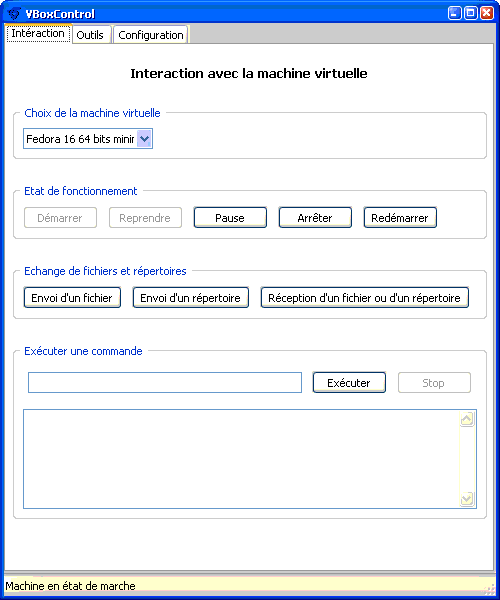
\includegraphics[scale=0.6]{img/Interface_solution_1.png}
	\caption{Interface graphique de la solution - Onglet 1 : l'interaction}
	\label{Interface graphique de la solution - Onglet 1 : l'interaction}
\end{figure}


Il faut tout d'abord choisir une machine virtuelle parmi la liste des machines installées sur la machine hôte.
Si l'utilisateur possède une machine virtuelle, utilisant Linux et paramétrée correctement, il pourra aussi utiliser l'interface graphique pour la contrôler.

Une fois la machine choisie, les différents boutons et onglets s'activent, et l'on peut utiliser l'interface.
\\


On peut ensuite allumer, éteindre, mettre en pause, ou redémarrer la machine virtuelle.

La machine virtuelle s'exécute en tâche de fond, c'est à dire que la fenêtre visible sur la capture d'écran \ref{Screenshot Virtualisation} n'apparait pas.
\\


Des boutons permettent d'échanger des fichiers ou des répertoires avec la machine virtuelle.
Une fenêtre de dialogue (objet de wxPython qui affiche l'arborescence de Windows) propose à l'utilisateur de choisir le fichier ou répertoire à envoyer, ou le répertoire cible de la réception.
Mais il est impossible de proposer la même fenêtre pour choisir le fichier ou répertoire à recevoir, ou le répertoire cible lors de l'envoi.
Il faut donc rentrer manuellement le chemin.
\\


En cas de problème, ou de besoin particulier, l'utilisateur peut exécuter des commandes.
Un thread\footnote{Thread : tâche qui s'exécute en parallèle.} va les exécuter à l'aide de Plink (voir partie \ref{Contrôle de la machine virtuelle} qui détail le contrôle de la machine virtuelle).
L'affichage retournée par la ou les commandes est reportée "en direct" dans la fenêtre pour informer l'utilisateur. 
\\



%%%%%%%%%%%%%%%%%%%%%%%%%%%%%%%%%%%%%%%%%%%%%%%%%%%%%%%%%%%%%%%%%%%%%%%%%%%%%%%%%%%%%%%%%%%%%%%%%%%%

\subsubsection{Les outils}

\begin{figure}[!h]
	\center
	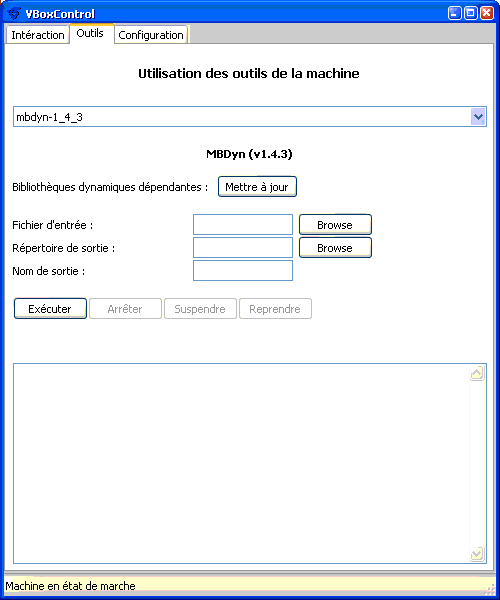
\includegraphics[scale=0.6]{img/Interface_solution_2.png}
	\caption{Interface graphique de la solution - Onglet 2 : les outils}
	\label{Interface graphique de la solution - Onglet 2 : les outils}
\end{figure}


Chaque outil possède son interface spécifique, présente dans un fichier qui lui est dédié.
L'ensemble de ces fichiers est rassemblé dans un répertoire spécifique.
Lors du chargement de l'interface graphique, ces morceaux d'interface sont chargés dynamiquement.

On peut ensuite choisir l'outil désiré dans la liste déroulante, qui affichera son interface juste en dessous.
\\


Lors de l'exécution d'un outil, la démarche est généralement la même pour tous :
\begin{enumerate}
	\item branchement du disque virtuel de l'outil sur la machine virtuelle ;
	\item montage du disque, dans un répertoire spécifique ;
	\item envoi des fichiers d'entrée dans la machine virtuelle ;
	\item exécution du programme, en spécifiant les différentes options ;
	\item réception des résultats sur la machine hôte ;
	\item démontage du disque ;
	\item débranchement du disque virtuel de la machine virtuelle ;
\\
\end{enumerate}


Pour régler le problème de dépendance expliqué dans la partie \ref{Compilation statique}, un bouton est mis à disposition de l'utilisateur pour installer les différents paquets nécessaires au fonctionnement de l'outil sélectionné.
\\


Dans la capture d'écran \ref{Interface graphique de la solution - Onglet 2 : les outils}, il s'agit de l'outil MBDyn qui requiert de spécifier trois options :
\begin{enumerate}
	\item le fichier d'entrée, qui contient les différentes données qui seront traitées ;
	\item le répertoire de sortie, dans lequel les résultats seront générés ;
	\item le nom des fichiers générés, qui porteront une extension différente pour les différencier.
\end{enumerate}
Selon l'outil l'interface peut être totalement différente, car les options ne sont pas les mêmes.
\\



%%%%%%%%%%%%%%%%%%%%%%%%%%%%%%%%%%%%%%%%%%%%%%%%%%%%%%%%%%%%%%%%%%%%%%%%%%%%%%%%%%%%%%%%%%%%%%%%%%%%

\subsubsection{La configuration}

\begin{figure}[!h]
	\center
	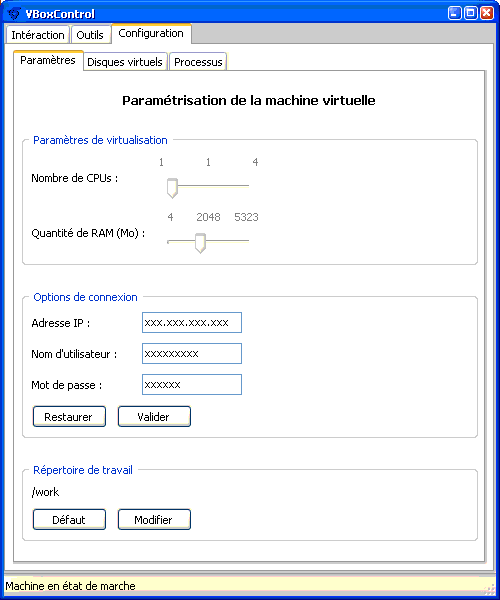
\includegraphics[scale=0.6]{img/Interface_solution_3.png}
	\caption{Interface graphique de la solution - Onglet 3 : la configuration}
	\label{Interface graphique de la solution - Onglet 3 : la configuration}
\end{figure}


Cet onglet permet d'effectuer certains réglages de la machine virtuelle.
Ils ne sont pas exhaustifs, et l'on pourra y ajouter d'autres options dans une version future.
\\

Il est possible de régler le nombre de cœurs, et la quantité de mémoire vive allouée à la machine virtuelle, lorsque celle-ci est éteinte.

Plink pour l'envoi de commandes (partie \ref{Contrôle de la machine virtuelle}) et Pscp pour l'échange de fichiers (partie \ref{Échange par SSH}) nécessitent une adresse IP, un nom d'utilisateur, ainsi qu'un mot de passe pour établir la connexion.
Il est possible de modifier ces options de connexion mais il est nécessaire qu'elles soient correctes pour que cela fonctionne.
\\ 


Deux sous-onglets "Disques virtuels" et "Processus", permettent respectivement d'ajouter ou retirer un disque virtuel de la machine, et de tuer ou mettre en pause un processus de la machine virtuelle.
\\




%%%%%%%%%%%%%%%%%%%%%%%%%%%%%%%%%%%%%%%%%%%%%%%%%%%%%%%%%%%%%%%%%%%%%%%%%%%%%%%%%%%%%%%%%%%%%%%%%%%%
%%%%%%%%%%%%%%%%%%%%%%%%%%%%%%%%%%%%%%%%%%%%%%%%%%%%%%%%%%%%%%%%%%%%%%%%%%%%%%%%%%%%%%%%%%%%%%%%%%%%
%%%%%%%%%%%%%%%%%%%%%%%%%%%%%%%%%%%%%%%%%%%%%%%%%%%%%%%%%%%%%%%%%%%%%%%%%%%%%%%%%%%%%%%%%%%%%%%%%%%%

\subsection{Ses limites}

Les différentes méthodes développées (voir partie \ref{Manipulation des machines virtuelles}) semblent assez lentes, car en effectuant certaines actions, l'interface se fige quelques secondes.
Par exemple, pour afficher la liste des processus de la machine virtuelle dans l'onglet "Configuration", il faut environ deux secondes pour que la liste soit rafraichie.
\\


Il serait possible de "Threader" les commandes, mais l'application serait beaucoup plus complexe à développer.
Pour augmenter les performances, l'utilisation de LibVirt ou du SDK de VirtualBox pourrait permettre des performances meilleures (détaillées en partie \ref{Paramétrisation de la machine virtuelle}).

Faute de temps, j'ai préféré me concentrer sur des points plus importants du projet, en utilisant des techniques moins performantes mais fonctionnelles.
\\





%%%%%%%%%%%%%%%%%%%%%%%%%%%%%%%%%%%%%%%%%%%%%%%%%%%%%%%%%%%%%%%%%%%%%%%%%%%%%%%%%%%%%%%%%%%%%%%%%%%%
%%%%%%%%%%%%%%%%%%%%%%%%%%%%%%%%%%%%%%%%%%%%%%%%%%%%%%%%%%%%%%%%%%%%%%%%%%%%%%%%%%%%%%%%%%%%%%%%%%%%
%%%%%%%%%%%%%%%%%%%%%%%%%%%%%%%%%%%%%%%%%%%%%%%%%%%%%%%%%%%%%%%%%%%%%%%%%%%%%%%%%%%%%%%%%%%%%%%%%%%%
%%%%%%%%%%%%%%%%%%%%%%%%%%%%%%%%%%%%%%%%%%%%%%%%%%%%%%%%%%%%%%%%%%%%%%%%%%%%%%%%%%%%%%%%%%%%%%%%%%%%
%%%%%%%%%%%%%%%%%%%%%%%%%%%%%%%%%%%%%%%%%%%%%%%%%%%%%%%%%%%%%%%%%%%%%%%%%%%%%%%%%%%%%%%%%%%%%%%%%%%%

\section{Déploiement de la solution}

La solution est scindée en plusieurs parties :
\begin{itemize}
	\item La machine virtuelle et ses outils :
		\begin{itemize}
			\item Le système d'exploitation (Linux) est installé sur un disque virtuel assez volumineux, car il contient l'ensemble des bibliothèques dynamiques, et va grandir au fur et à mesure de son utilisation.
Lors de la première utilisation, la taille est minimale car aucune bibliothèque (hormis celles installées par défaut) n'est installée.
Ce disque virtuel est déployé une seule fois, car c'est la base de la solution sur laquelle viendront s'ajouter les outils ;
			\item Les outils sont installés sur des disques virtuels distincts et individuels.
Ainsi, lorsqu'un nouvel outil (demandé par un utilisateur) est disponible, seul son disque virtuel sera déployé sur les différents ordinateurs.
L'ensemble des outils sera situé dans un répertoire dédié.
		\end{itemize}
	\item L'interface graphique :
		\begin{itemize}
			\item La base de l'interface graphique utilisateur devrait, comme le disque virtuel du système, être déployé une seule fois, lors de la mise en place de la solution ;
			\item Les différents fichiers, contenant l'interface graphique de l'outil, seront aussi installés dans un répertoire spécifique.
Lors du déploiement d'un nouvel outil, son fichier sera ajouté au répertoire pour qu'il puisse apparaitre dans l'interface graphique.
\\
		\end{itemize}
\end{itemize}


Le déploiement s'effectuera de manière optimale, facilitant aussi les futures mises à jour ou ajouts d'outils.